%%%%                %%%%
%%%% BASES TEÓRICAS %%%%
%%%%                %%%%

\chapter{Bases teóricas}
\label{chap:bases-teoricas}

\lettrine{E}{l} objetivo de este capítulo es sentar las bases tecnológicas y teóricas sobre las que se ha llevado a cabo el proyecto. En particular, se expone de qué manera se consiguen las coordenadas de las palabras y qué tecnologías intervienen para la obtención de la salida en formato estructurado.

Las aplicaciones comerciales utilizan las ubicaciones para seleccionar contenidos relevantes. Lo habitual es que el usuario pueda marcar rectángulos sobre las páginas y que los procesos de extracción y verificación únicamente tengan en cuenta estas áreas. Para poder hacer esto se necesitan las localizaciones de las palabras, pares clave-valor, tablas, etc. Entre los PDF manejados para la elaboración de este trabajo hay dos categorías importantes: aquellos que tienen texto directamente extraíble y otros donde cada página es una imagen. El primer caso es el habitual en los PDF generados con procesadores de textos u otros software. Se puede comprobar fácilmente si un PDF contiene texto directamente extraíble abriendo el documento con un visor y realizando la selección con el ratón. Si la operación es posible, se puede evitar hacer OCR del documento y obtener una versión del texto sin los errores derivados del Reconocimiento Óptico.

\section{Software para la manipulación de PDF}

Existen librerías y también aplicaciones capaces de manipular ficheros PDF para extraer texto, imágenes, reordenar páginas y otras muchas posibilidades. Para los objetivos del proyecto, se necesita una herramienta capaz de extraer el texto pero también sus coordenadas sobre el documento. Se revisaron varias alternativas, como PDFBox 
\footnote{\url{https://pdfbox.apache.org/}}, Win2PDF 
\footnote{\url{https://www.win2pdf.com/doc/command-line-extract-text-pdf.html}}, ebook-convert 
\footnote{\url{https://manual.calibre-ebook.com/es/generated/es/ebook-convert.html}}, que forma parte de la aplicación Calibre, y \verb|pdftotext| 
\footnote{\url{https://poppler.freedesktop.org/}}. Únicamente esta última ofrece la posibilidad de generar las localizaciones necesarias.

La implementación original de esta utilidad fue realizada por Glyph \& Cog \footnote{\url{http://www.glyphandcog.com/}}, autores del visor Xpdf. En el año 2005 apareció la librería Poppler a partir del fork de la versión 3.0.3 de Xpdf. Esta es la implementación disponible mayormente en las distribuciones Linux. Por ejemplo, en Ubuntu se puede instalar con el paquete \verb|poppler-utils| e incluye otras muchas herramientas relacionadas.

Cuando se invoca la herramienta con el parámetro \verb|-bbox| se genera una salida en lenguaje XHTML. Esta variante del HTML tiene la ventaja de ser admitida por cualquier parser XML. Se identifican tags para los elementos que representan bloques, lineas y palabras. En cada uno se informa con cuatro valores de la localización del rectángulo que engloba al elemento: \emph{xMin}, \emph{xMax}, \emph{yMin}, \emph{yMax}. La generación de información de coordenadas o bounding box, además del texto, existe gracias a una aportación al proyecto en el año 2010 de Kenneth Berland. 

\begin{figure}[hp!]
    \centering
    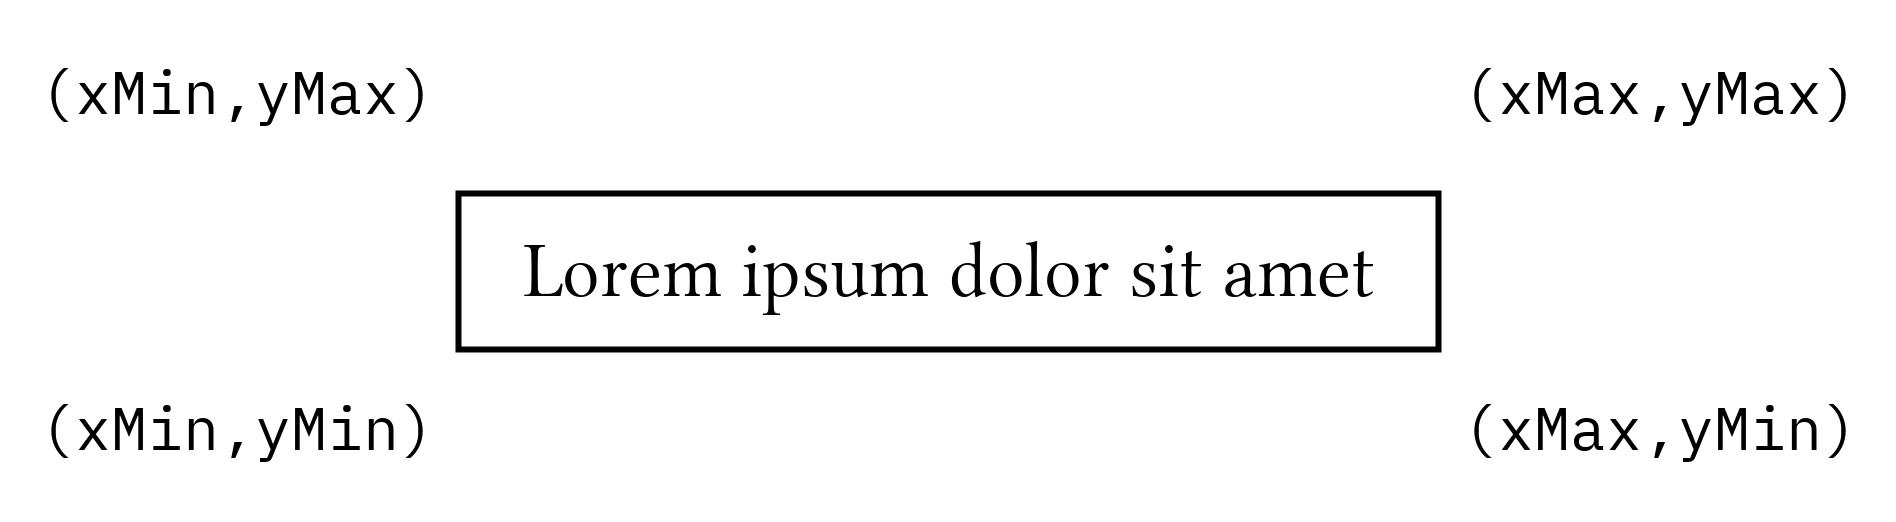
\includegraphics[width=0.75\textwidth]{imaxes/c-bases-teoricas/correspondencia-coordenadas-bounding.png}
    \caption{Correspondencia de las coordenadas en una bounding box}
    \label{fig:bounding-box}
\end{figure}

Una limitación común en todas estas utilidades consiste en no respetar el layout del texto, tal como aparece en el documento original. Esto implica que algunos elementos pueden aparecer antes que otros en la información extraída. Otro problema es que hay palabras que aparecen con caracteres extraños intercalados, o espacios. Las anomalías comentadas no son visibles en el PDF. Estas limitaciones se derivan del propio funcionamiento del formato PDF.

\section{El formato PDF}

PDF es un formato digital para la creación de documentos. Fue introducido por Adobe Systems en 1993. En los siguientes años, el uso de este formato se extendió por toda la sociedad, tanto en el ámbito público como en el privado. En el año 2008, la ISO publicó el estándar 32000-1, tomando como base especificación de PDF en su versión 1.7, creada y liberada por Adobe. Posteriormente se publicó la versión 2.0 como ISO 32000-2 en el año 2017 y más recientemente una actualización en el año 2020. PDF es un modelo de representación de imágenes que deriva del lenguaje PostScript, también desarrollado por Adobe. En PDF, el modelo de imagen admite gráficos y texto de forma independiente al dispositivo de salida. 

% TODO Considerar si añadir más información de PostScript.

\subsection{Almacenamiento de información}

Un PDF no es un fichero de texto, es un formato binario de 8 bits con una estructura interna determinada. Sus elementos básicos son los objetos. Cualquier información que se visualice en el documento existirá realmente como un objeto dentro del archivo. Estos objetos están serializados dentro del fichero y pueden ser de alguno de los siguientes nueve tipos:

\begin{enumerate}
    \item \textbf{Null}: se utiliza para indicar la ausencia de un valor.
    \item \textbf{Boolean}: indica los valores de verdad, true o false.
    \item \textbf{Integer}: representa valores enteros. Puede aparecer como \verb|1|, \verb|+2|, \verb|-100|.
    \item \textbf{Real}: representa valores decimales y puede aparecer como \verb|0,05|, \verb|.25|, \verb|-3,1415|.
    \item \textbf{Name}: son secuencias únicas dentro del fichero, comienzan con una barra. Por ejemplo: \verb|/Type|, \verb|/ThisIsAName|.
    \item \textbf{String}: puede ser de 4 tipos:
    \begin{itemize}
        \item ASCII: bytes codificados en ASCII.
        \item PDFDocEncoded: bytes codificados con la codificación PDFDocEncoding.
        \item Text: bytes codificados en PDFDocEncoding o UTF-16BE.
        \item Date: utilizado para fechas. Se codifican en ASCII con un patrón de fecha. \footnote{En concreto, el patrón para las fechas es: D:YYYYMMDDHHmmSSOHH’mm.}.
    \end{itemize}
    \item \textbf{Array}: es una colección heterogénea de objetos. Se escriben entre corchetes: \verb|[ 0 20 (E) ]|.
    \item \textbf{Dictionary}: es una tabla asociativa que contiene pares clave/valor. Los valores anidados están permitidos y es utilizado para crear la jerarquía de todos los objetos del documento. Para indicar el comienzo y fin se utilizan los símbolos \verb|<<| y \verb|>>|. Las claves se indican con valores de tipo Name.
    \item \textbf{Streams}: son secuencias de bytes de 8 bits sin límite de tamaño. Son utilizados para almacenar cualquier información binaria, por ejemplo imágenes, ficheros JSON o tipografías. Los stream tienen como preámbulo un diccionario de propiedades del stream. Este diccionario siempre debe contener, al menos, la clave \verb|/Length| que indica en bytes el tamaño del stream. Otra clave importante es \verb|/Filter|. \verb|/Filter| indica que la información está comprimida o codificada. Las imágenes se suelen codificar como DCTDecode o JPXDe que son versiones diferentes del formato JPEG. Para otro tipo de datos está disponible el algoritmo FlateDecode, similar a  DEFLATE, el mismo utilizado en los ficheros ZIP.
\end{enumerate}

Los objetos presentados hasta el momento son los objetos directos. Los objetos directos tienen el valor almacenado en el propio objeto. También existen los objetos indirectos que se referencian indirectamente y el consumidor tiene que saltar a otra posición en el fichero. Los objetos indirectos tienen un identificador único dentro del fichero. Las referencias son de la forma: \verb|/ObjIndirecto  5 0 R|.

\subsection{Estructura física}

La estructura física de un fichero está dividida en cuatro partes, tal como se muestra en la Figura \ref{fig:secciones-pdf}: Header, Body, Cross-Reference Table y Trailer. El Header tiene al menos dos líneas. La primera se utiliza para indicar que el fichero es un PDF y la versión del estándar que le corresponde. La segunda es simplemente un separador: \verb|%%EOF|. 

\begin{figure}[hp!]
    \centering
    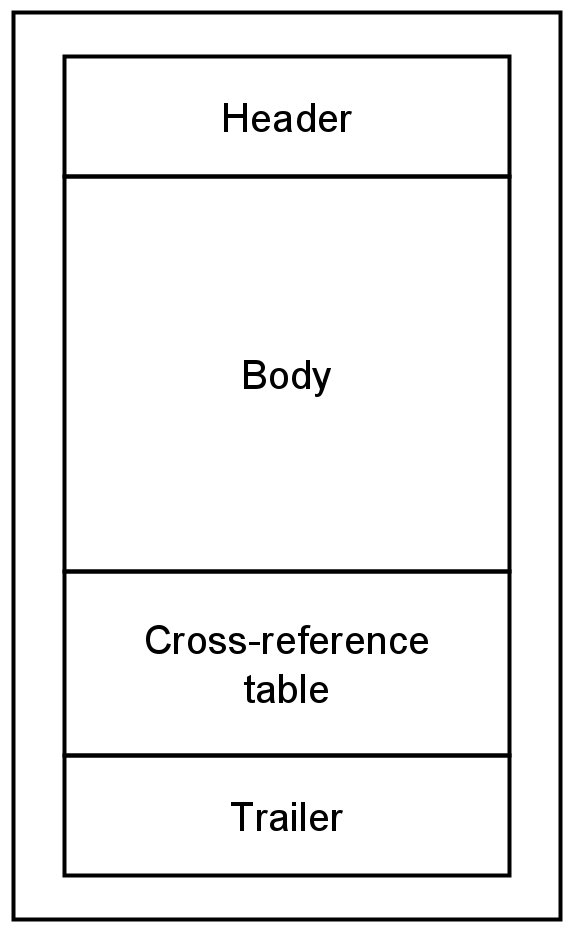
\includegraphics[width=0.3\textwidth]{imaxes/c-bases-teoricas/secciones-de-un-pdf.png}
    \caption{Las cuatro secciones de un PDF}
    \label{fig:secciones-pdf}
\end{figure}

El Trailer es un objeto de tipo diccionario. Contiene claves y valores que aportan información a nivel de documento. Hay dos claves especialmente importantes, /Size que indica el número de entradas de la Cross-Reference Table y /Root que apunta al objeto que contiene el comienzo del Catálogo. El Body contiene el objeto del Catálogo y todos los demás objetos que conforman el contenido del fichero PDF. La Cross-Reference Table es un índice de todos los objetos indirectos del PDF. Se utiliza para implementar la navegación sobre el fichero. Contiene la información necesaria para poder realizar saltos a la posición donde se encuentra el objeto que se quiere leer. La versión tradicional tiene tres columnas y la secuencia de entradas hace referencia al número del objeto buscado. En el ejemplo, para encontrar el objeto 2, tercera entrada, hay que saltar hasta el byte 32800:

\begin{lstlisting}[caption={Entradas en la Cross-Reference Table},label=lst:cross-ref-table]
0000000000 65535 f
0000000009 00000 n
0000032800 00000 n
0000000203 00000 n
0000000298 00000 n
0000008654 00000 n
0000000335 00000 n
\end{lstlisting}

No existe una gran cantidad de herramientas visuales para explorar el árbol de objetos de un PDF, al menos fáciles de encontrar y gratuitas. En la Imagen \ref{fig:estructura-interna-pdf} se presenta una de ellas, PDFXplorer \footnote{\url{https://www.o2sol.com/pdfxplorer/overview.htm}}, con un ejemplo de documento cuyo único contenido es el texto \emph{Hola mundo!}. En la imagen se visualiza un fragmento del stream que alberga el texto, en particular las líneas 22 a 32, equivales a cada uno de los caracteres de la página. Alternativamente también se puede analizar un PDF de forma manual con herramientas simples en la línea de comandos \cite{filodej_blog_pdfstreamcontent}.

\begin{figure}
	\centering
	\begin{subfigure}[b]{0.29\textwidth}
		\centering
		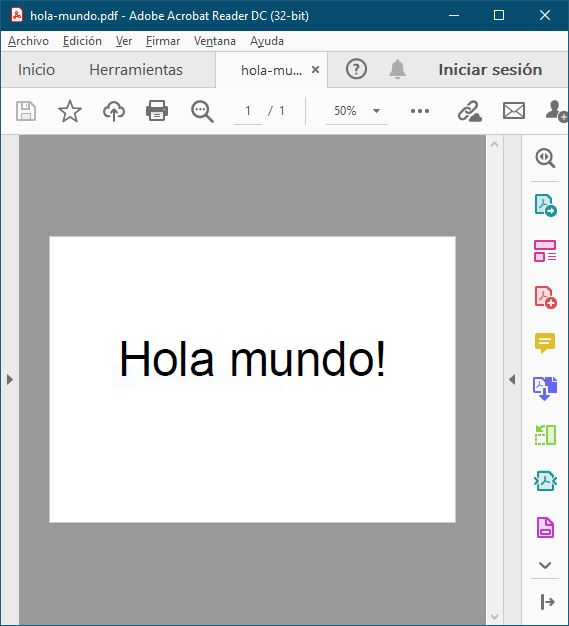
\includegraphics[width=\textwidth]{imaxes/c-bases-teoricas/hola-mundo-adobe-reader}
		\caption{PDF en Adobe Reader}
		\label{fig:hola-mundo-adobe-reader}
	\end{subfigure}
	\hfill
	\begin{subfigure}[b]{0.7\textwidth}
		\centering
		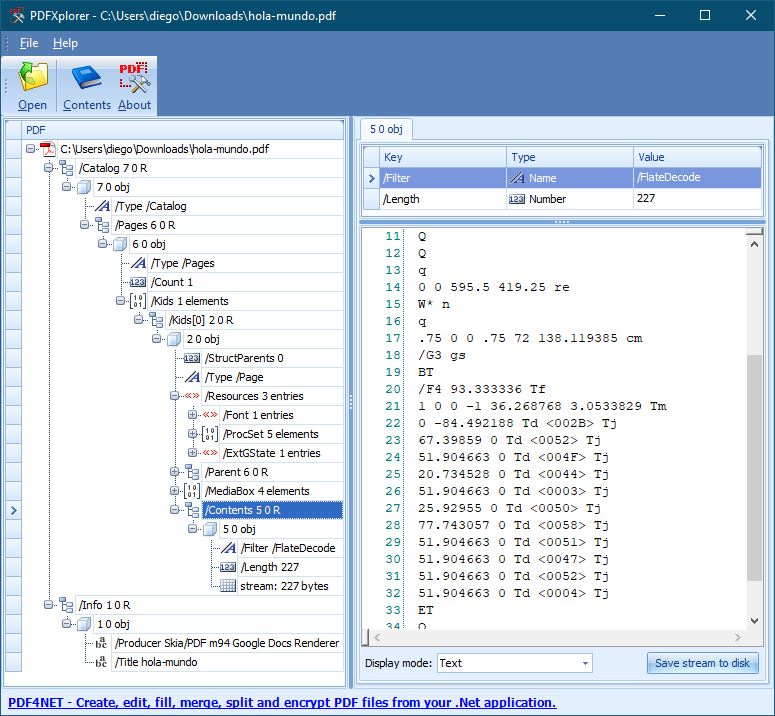
\includegraphics[width=\textwidth]{imaxes/c-bases-teoricas/hola-mundo-pdfxplorer}
		\caption{Árbol de objetos del PDF en PDFXplorer}
		\label{fig:hola-mundo-pdfxplorer}
	\end{subfigure}
	\caption{Elementos internos de un PDF simple}
	\label{fig:estructura-interna-pdf}
\end{figure}


% TODO Considerar hablar del catálogo o dejarlo para la parte de implementación.

\section{Representación de coordenadas en orígenes OCR}

La representación de las localizaciones de los elementos identificados por el proceso OCR es solo una parte de toda la información que se genera como salida de un motor OCR. Existen varias alternativas de formatos que se proponen como formatos abiertos con intención de favorecer su adopción. Es el caso de hOCR \cite{ocrRepres_hocr_breuel_spec}, ALTO \cite{ocrRepres_alto_spec}, PAGE \cite{ocrRepres_page_pletschacher_paper} y TEI \cite{ocrRepres_tei_project}. Los tres últimos emplean XML como base y definen las etiquetas necesarias. La transformación entre ellos es posible y existe al menos un proyecto capaz de hacerlo
\cite{ocrRepres_conversion_ocrFileformat}. hOCR es el formato de representación escogido para el proyecto, como se verá en la Sección \ref{sec:rec-optico-caracteres}.

\subsection{El microformato hOCR}

hOCR es un estándar abierto que utiliza HTML como base tecnológica. Se diseñó siguiendo los modelos de los microformatos \footnote{\url{http://microformats.org/}}. Los microformatos son una tecnología ligada al auge de los blogs durante el año 2004. Su objetivo es aportar significado semántico a construcciones HTML, que de otro modo no lo tendrían, ya que no forman parte como tal del lenguaje. El funcionamiento es sencillo, se incorporan a ciertos tags, atributos con la información necesaria. En el caso de hOCR, la especificación hace uso de etiquetas \verb|DIV| y \verb|SPAN| para los elementos. Para la información se utilizan atributos como \verb|class|, \verb|title| o \verb|style|. Uno de los motivos para basarse en HTML a la hora de diseñar el formato fue que este tiene soporte nativo para muchas de las características habituales en los documentos como el estilo, tipografías, espaciado, etc. Además, para ampliar las capacidades de representación se combina con CSS.

La especificación hOCR define tres tipos de marcado:

\begin{itemize}
    \item Un marcado a \textbf{nivel lógico} que permite definir las secciones de un documento como en una estructura de tipo árbol.
    \item Un segundo tipo de marcado para representar el \textbf{nivel tipográfico y de división entre páginas}. Tiene la capacidad de modelar el documento de forma  que sus elementos principales se trasladarían al formato impreso de forma correcta. Este modelo se apoya en los procesos habituales que consideran el documento como un conjunto de bloques y elementos que se deben trasladar a su posición correcta.
    \item Un ultimo tipo para el \textbf{nivel físico} representado por líneas, figuras, y las palabras. Es específico para la implementación de cada motor de OCR. 
\end{itemize}

El formato proporciona también información geométrica, posiciones, de las palabras y valores de confianza respecto a la calidad que el motor otorga al reconocimiento realizado.

\section{Reconocimiento Óptico de Caracteres}
\label{sec:rec-optico-caracteres}

Para realizar el Reconocimiento Óptico de Caracteres se seleccionó Tesseract \cite{ocr_tesseract_raysmithetal.TesseractocrTesseract2021}. Existen otros proyectos de fuente abierta que se pueden considerar:

\begin{itemize}
    \item \textbf{OCRopus} \cite{ocr_ocropus_ocropy_project}, \textbf{Kraken} y \textbf{Calamary} \cite{ocr_calamari_journal}: OCRopus es una colección de herramientas para el análisis, más que un producto final utilizable. Kraken y Calamary son dos derivaciones de OCRopus que proporcionan un producto final. Sin embargo los tres proyectos están enfocados en resolver el problema de reconocer textos históricos con tipografías clásicas. Revisando la documentación de los tres no se encontraron modelos preentrenados en castellano.
    \item \textbf{EasyOCR} (\cite{ocr_easyocr_official}, \cite{ocr_easyocr_project}) es la alternativa más viable. Es un proyecto que se actualiza regularmente y tiene soporte comercial. Como punto negativo destaca que aunque proporciona información de bounding-box, no sigue ninguno de los estándares comentados con anterioridad.
\end{itemize}

\textbf{Tesseract} \cite{ocr_tesseract_smith_paper} es un engine de código abierto y desarrollado inicialmente por Hewlett Packard \cite{ocr_tesseract_v4_release_notes} entre los años 1985 y 1995. Después de un periodo sin actividad, en el 2006 el proyecto fue recuperado por Google, que lo mantiene desde entonces. Hoy en día tiene soporte para más de cien idiomas y la red neuronal que emplea \footnote{Desde la versión 4, Tesseract utiliza una red LSTM. Esta es una red neuronal de tipo recurrente o RNN.} puede ser entrenada para casos específicos, si se necesita. Existe una amplia documentación en la web oficial, además, numerosos tutoriales en la red permiten familiarizarse con la herramienta. Es un proyecto bien conocido y de larga trayectoria.

\section{Detección de líneas en tablas}

Existen documentos que contienen tablas donde hay dibujadas rectas que separan dos líneas de contenido, esto se detalla más en la Sección \ref{sec:sobre-los-documentos}. La Transformada de Hough (\cite{hough_krishna_computerVision}, \cite{hough_grauman_presentation}) proporciona una manera automática de delimitar esos espacios.

Este algoritmo es una técnica de visión por computador utilizada para detectar figuras tales como líneas o círculos. Se puede aplicar a cualquier figura siempre que se conozca una ecuación paramétrica que la defina. A continuación se detalla el funcionamiento general del algoritmo.

Se utiliza como entrada la información obtenida al aplicar un detector de bordes en la imagen original. Si se considera un punto borde cualquiera, sobre él pueden pasar infinitas rectas. Estas rectas se pueden definir con la Ecuación \ref{hough-ecu-recta}.

\begin{equation}
    \label{hough-ecu-recta}
    y = a*x + b
\end{equation}

Reescribiendo la ecuación como,

\begin{equation}
b = -a*x + y
\end{equation}

es posible transformar cada punto borde al espacio de Hough y obtener una recta en dicho espacio.

Considerando dos puntos del espacio imagen (\ref{fig:hough-punto-imagen}), al trasladarlos al espacio Hough (\ref{fig:hough-intersection}) se puede calcular su intersección resolviendo el sistema de ecuaciones. Esta intersección proporciona los parámetros para construir, en el espacio imagen, la recta (\ref{fig:hough-recta-a-b}) que une ambos puntos.

\begin{figure}
    \centering
    \begin{subfigure}[b]{0.3\textwidth}
        \centering
        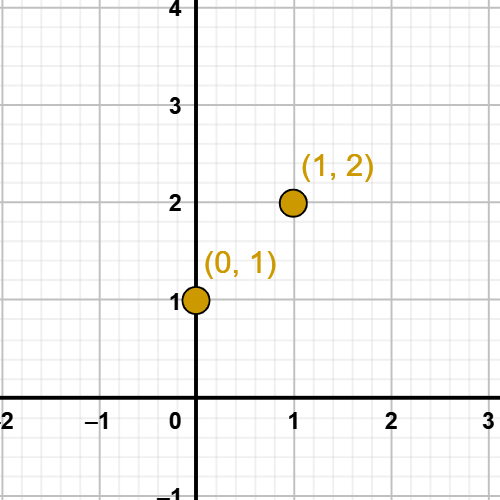
\includegraphics[width=\textwidth]{imaxes/c-bases-teoricas/hough-1}
        \caption{Dos puntos borde en el espacio imagen}
        \label{fig:hough-punto-imagen}
    \end{subfigure}
    \hfill
    \begin{subfigure}[b]{0.3\textwidth}
        \centering
        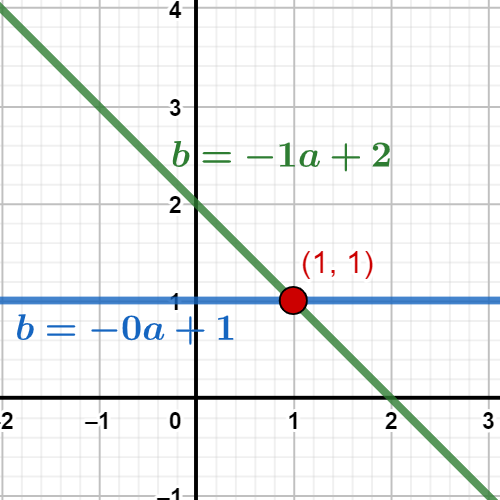
\includegraphics[width=\textwidth]{imaxes/c-bases-teoricas/hough-2}
        \caption{Rectas e intersección en el espacio Hough}
        \label{fig:hough-intersection}
    \end{subfigure}
    \hfill
    \begin{subfigure}[b]{0.3\textwidth}
        \centering
        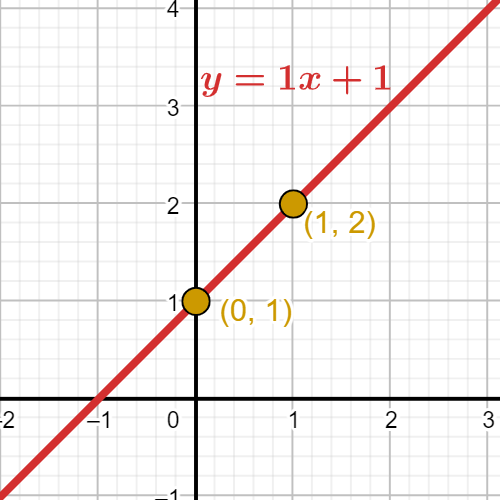
\includegraphics[width=\textwidth]{imaxes/c-bases-teoricas/hough-3}
        \caption{Recta que une ambos punto en el espacio imagen}
        \label{fig:hough-recta-a-b}
    \end{subfigure}
\end{figure}

El procedimiento general del algoritmo es como sigue:

\begin{enumerate}
    \item Se cuantiza el espacio de Hough. La cuantización divide el espacio en celdas.
    \item Se toma cada par de puntos de la imagen borde.
    \begin{enumerate}
        \item Se calcula su intersección.
        \item Se busca la celda donde coincide el punto intersección.
        \item Se aumenta en uno el recuento de votos de esta celda.
    \end{enumerate}
    \item Al finalizar, las celdas más votadas son las candidatas a ser líneas reales.
\end{enumerate}

\section{Análisis léxico y sintáctico}

\subsection{Introducción}

Como parte del proyecto se ha desarrollado una herramienta que utiliza análisis léxico y sintáctico para crear una salida estructurada, acorde a los requisitos. Estas dos tareas de análisis son etapas habituales para los compiladores de lenguajes de programación. Los siguientes apartados explican algunos de los aspectos principales para poder entender como se han aplicado en la implementación (en el Capítulo \ref{chap:implemetación}).

\subsection{Conceptos básicos}

En primer lugar se presentan algunos de los conceptos elementales que serán citados en el resto de la memoria.

\begin{itemize}
    \item Un \textbf{lenguaje} es un conjunto de cadenas de longitud finita creadas a partir de un alfabeto finito.
    \item Los \textbf{alfabetos} son colecciones finitas de símbolos.
    \item Las \textbf{palabras} o \textbf{cadenas} son secuencias de símbolos tomados de un alfabeto. La cadena vacía es aquella cadena que carece de símbolos. Se representa habitualmente con el símbolo $\epsilon$.
    \item Las \textbf{producciones} son reglas de sustitución que al aplicarse generan cadenas en el lenguaje.
    \item Un \textbf{token} es la unidad mínima que se caracteriza por aportar significado léxico. Por ejemplo, en un lenguaje de programación cualquier palabra reservada es un token. Como también lo son los caracteres de los operadores matemáticos. Se les llama también símbolos terminales.
    \item El \textbf{axioma} en una gramática es el elemento desde el que se construyen todos los árboles de derivación en dicha gramática
    \item Los \textbf{símbolos no terminales} son aquellos símbolos que deben ser sustituidos por otros para generar totalmente una cadena.
    \item Un \textbf{árbol de derivación} es la representación gráfica que muestra la secuencia de transformaciones sucesivas que son necesarias para obtener una cadena particular, partiendo desde el axioma de una gramática.
\end{itemize}

\subsection{Teoría de Autómatas y Lenguajes Formales}

La Teoría de autómatas y los Lenguajes Formales son dos de los pilares que definen lo que un ordenador es capaz de hacer y qué cosas no son computables. Es la base científica sobre la que se construyen los compiladores. Estas herramientas son capaces de transformar código fuente, escrito en un lenguaje de programación, en otro lenguaje que el ordenador es capaz interpretar.

% lenguajes

Los Lenguajes Formales son aquellos donde las reglas para unir los símbolos del lenguaje están definidas formalmente. Las palabras en los lenguajes se forman a partir de alfabetos, de tal manera que, realizando combinaciones de símbolos presentes en el alfabeto es posible construir cadenas que pertenecerán al lenguaje y también otras muchas que no pertenecen. 

% gramáticas

La definición formal viene dada por las Gramáticas Formales. Estas indican como construir cadenas que son válidas según las reglas sintácticas. Las gramáticas contienen conjuntos de reglas de transformación o reglas de producción que se aplican sucesivamente hasta obtener la palabra deseada. Cuando no existe una combinación de reglas que permita obtener una cadena determinada se conoce que esa cadena no pertenece al lenguaje.

Las reglas son de la forma $A\rightarrow S$ y pueden estar formadas por símbolos terminales y no terminales \footnote{Por consenso, los símbolos no terminales se utilizan en mayúscula y en minúscula los terminales, en Bison sin embargo el criterio es el opuesto.}. Este es un ejemplo de gramática:
\begin{center}
$S\rightarrow AB$ (regla 1) \\
$A\rightarrow aA$ (r. 2) \\
$A\rightarrow a$ (r. 3) \\
$B\rightarrow aB$ (r. 4) \\
\end{center}

Cuando se aplica una sustitución, se parte del lado derecho y se cambia por los símbolos del lado izquierdo de la producción. Con la gramática anterior se puede construir la palabra \verb|aab| partiendo del axioma y aplicando sucesivamente cuatro transformaciones, reglas 1, 4, 2 y 3 de la gramática:

\begin{center}
$S\Rightarrow AB\Rightarrow Ab \Rightarrow AaB \Rightarrow aab$
\end{center}

% autómatas

Los primeros autómatas fueron construidos en la Grecia clásica como pequeños artefactos capaces de moverse o actuar por si mismos. La Teoría de Autómatas trata de modelos matemáticos, o máquinas abstractas, capaces de reconocer un lenguaje formal. La Máquina de Turing es uno de estos modelos.

En su visión más inmediata, un autómata, es un diagrama que sirve para encontrar las palabras de un lenguaje. Se utiliza un grafo dirigido al que se le aporta información adicional. Los nodos del grafo son los estados e indican en qué punto del análisis de la cadena se encuentra. Las aristas van etiquetadas con caracteres del alfabeto y se llaman transiciones.

Un autómata especifica un lenguaje como el conjunto de aquellas cadenas que lo llevan del estado inicial a alguno de los estados finales o de aceptación. Al mismo tiempo un autómata puede ser visto como un generador de las cadenas de un lenguaje, si se comienza con la cadena vacía y se añaden símbolos según se recorren las transiciones, hasta llevar al autómata a un estado de aceptación.

A partir del diagrama de estados del autómata es posible obtener expresiones de la forma $S\rightarrow A$ que representan las  transiciones del autómata y se pueden aplicar como reglas de sustitución para la generación de cadenas.

% unión de conceptos

Queda por tanto clara la relación existente entre las gramáticas, los lenguajes y los autómatas. Una gramática proporciona las reglas para construir todas las palabras que pertenecen a un lenguaje. El autómata es el modelo matemático abstracto capaz de recibir cadenas del lenguaje y decidir si son válidas para una gramática.

% jerarquía Chomsky

Noam Chomsky es un investigador destacado en el ámbito de los lenguajes naturales y formales. En la década de los años 50 del siglo XX estaba estudiando el funcionamiento de la construcción de los lenguajes naturales y realizó aportaciones en el ámbito de las gramáticas formales.

Una de estas aportaciones se conoce como la jerarquía de Chomsky. Establece cuatro niveles de tipos de gramáticas dependiendo de la forma de sus reglas de producción o, equivalentemente, de lo restrictivas que sean a la hora de definir lenguajes. En la Imagen \ref{fig:niveles-chomsky} se puede ver las gramáticas en la jerarquía ampliada con los autómatas y lenguajes asociados.

\begin{figure}[hp!]
    \centering
    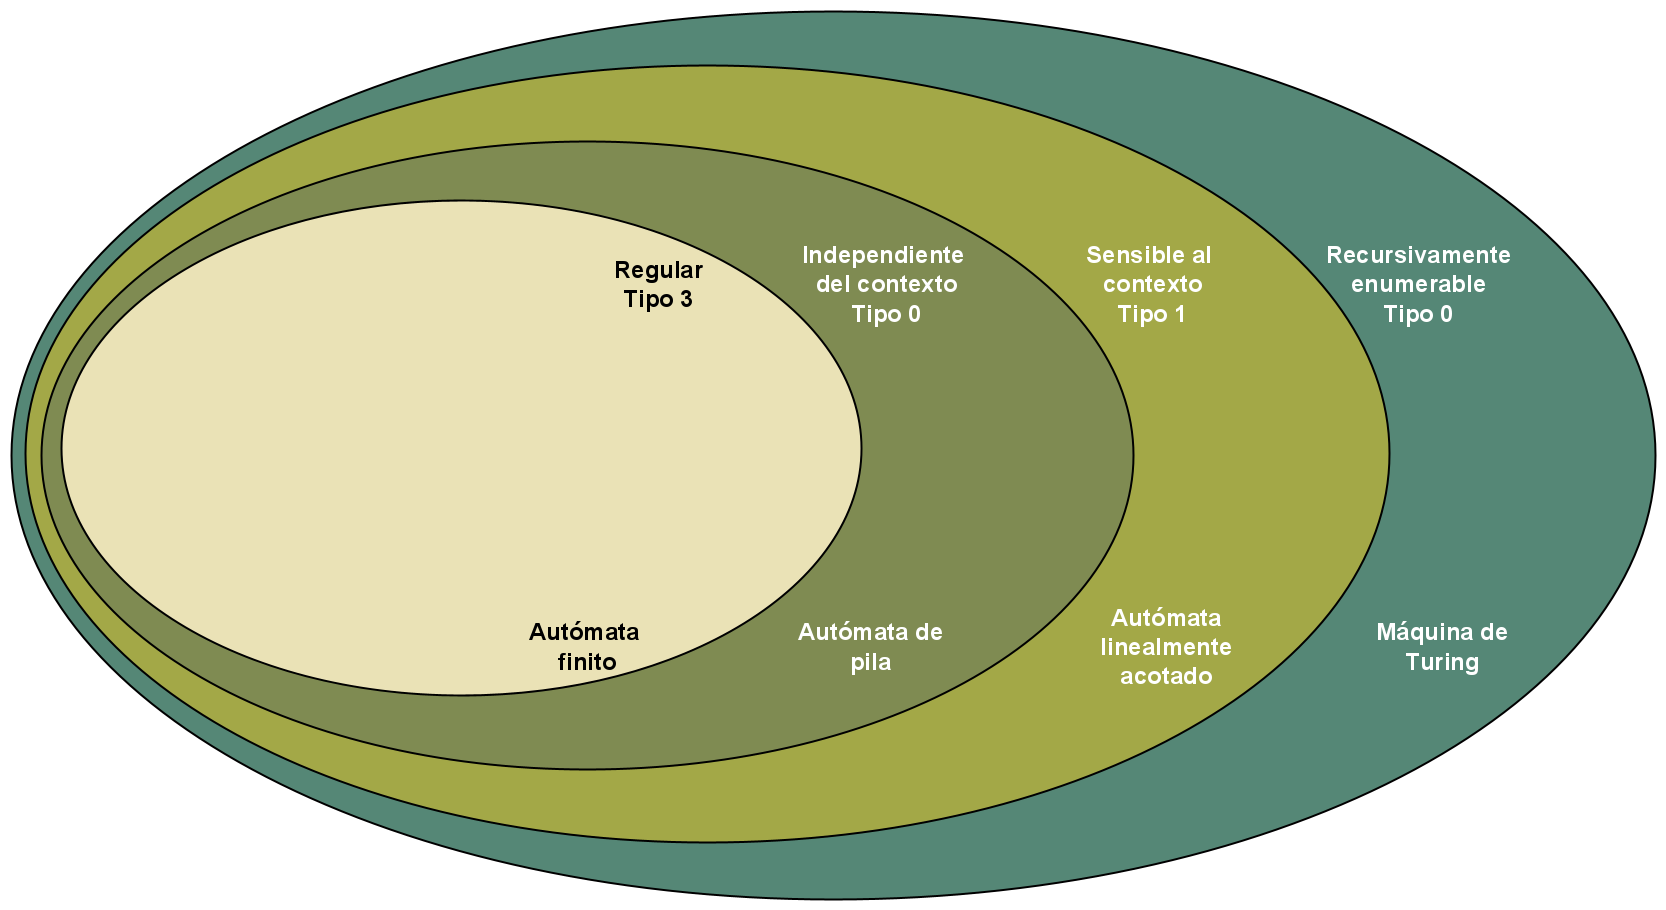
\includegraphics[width=1.0\textwidth]{imaxes/c-bases-teoricas/niveles-chomsky.png}
    \caption{Jerarquía de Chomsky}
    \label{fig:niveles-chomsky}
\end{figure}

% tipos de gramáticas

En la jerarquía de Chomsky se definen cuatro tipos de gramáticas. Comenzando con las más restrictivas respecto a la cantidad de lenguajes que son capaces de generar, están las gramáticas de Tipo 3 o Regulares. La forma de las reglas es:

\begin{center}
$A\rightarrow a$ o bien $A\rightarrow aB$
\end{center}

Se permiten también reglas que generen la cadena vacía, $A\rightarrow\epsilon$. Este tipo de gramáticas generan los mismos tipos de lenguajes que se pueden describir con las expresiones regulares.

Las gramáticas de Tipo 2 o Gramáticas Independientes del Contexto tienen producciones de la forma 

\begin{center}
$A\rightarrow \beta$
\end{center}

donde A es un no terminal y $\beta$ es una cadena que puede contener terminales y no terminales. Estas gramáticas son reconocidas por un autómata de pila, como el caso de Bison, que se explica en la Página \pageref{automatas-pila}. Estas son las gramáticas empleadas habitualmente en los lenguajes de programación.

La siguiente categoría son las Gramáticas Sensibles al Contexto o gramáticas de Tipo 1. En este caso, las reglas en forma normal son:

\begin{center}
$\alpha A\beta\rightarrow \alpha\gamma\beta$
\end{center}

de tal manera que A es un no terminal, $\alpha, \beta$ y $\gamma$ son cadenas de terminales y no terminales. Además $\alpha$ y $\beta$ pueden ser vacíos mientras que $\gamma$ no.
Estos lenguajes son reconocidos por una Máquina de Turing con una cinta de memoria acotada o limitada.

Las gramáticas más generales son las gramáticas de Tipo 0 o No Restringidas. Los lados izquierdos de las reglas pueden estar formados por cualquier combinación de terminales y no terminales, siempre y cuando contengan algún símbolo terminal. Sobre el lado derecho no existen restricciones.

Todos los lenguajes hasta aquí comentados son recursivamente enumerables, ya que existe para todos ellos una Máquina de Turing que acepta y se detiene con cualquier cadena del lenguaje. Pero, si la cadena no pertenece, puede parar y rechazar o bien iterar indefinidamente.

Sin formar parte de la jerarquía, existe otra categoría intermedia entre los sensibles al contexto y los recursivamente enumerables, son los lenguajes recursivos. En estos, se requiere que la Máquina de Turing pare en todos los casos, por este motivo se los conoce como lenguajes decidibles.

Los lenguajes regulares, Independientes del Contexto y los Sensibles al contexto son, a su vez, Recursivos.

\subsection{Notación BNF}

La notación Backus-Naur se utiliza para describir una gramática. Fue desarrollada por John Backus para el lenguaje Fortran y mejorada por Peter Naur para poder describir el lenguaje Algol 60.

En el Listado \ref{lst:ejemplo-gramatica-bnf} se muestra una pequeña gramática. Los símbolos \verb|::=| deben leerse \emph{se define como}. Para indicar alternativa, \emph{or}, se utiliza una barra vertical "|".

\begin{lstlisting}[caption={Gramática en notación BNF},label=lst:ejemplo-gramatica-bnf]
numero ::= val
         | val '.' val
val    ::= n
         | n val
n      ::= '0' | '1' | '2' | '3' | '4'
         | '5' | '6' | '7' | '8' | '9'
\end{lstlisting}

\begin{figure}[hp!]
    \centering
    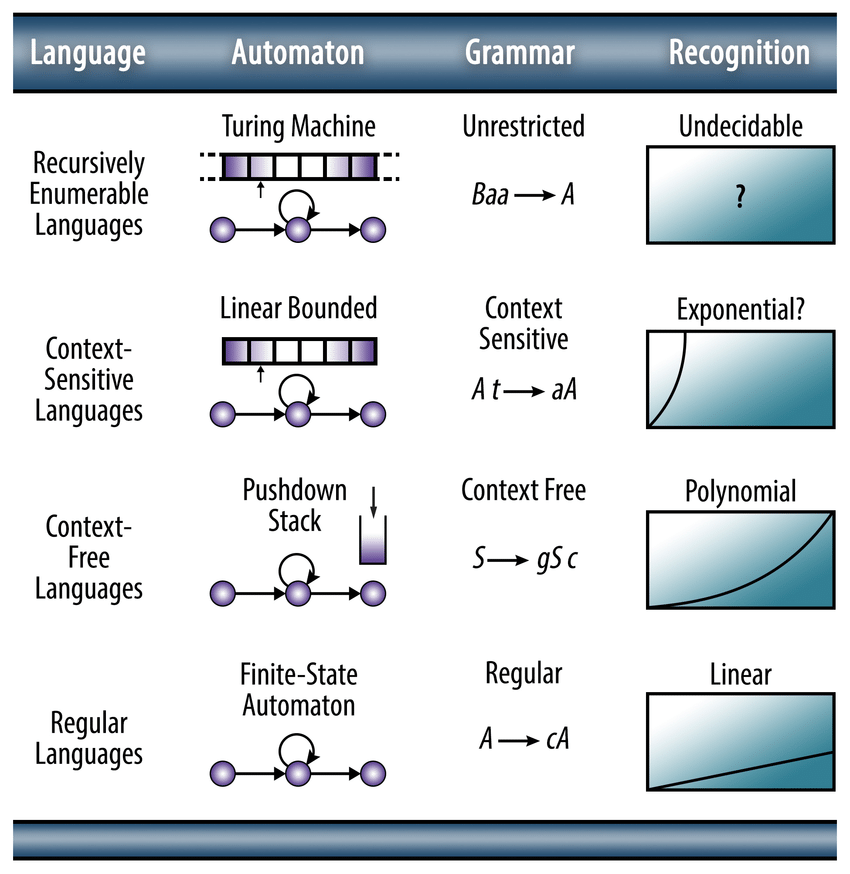
\includegraphics[width=0.6\textwidth]{imaxes/c-bases-teoricas/hauser-2016.png}
    \caption{Comparativa de los 4 modelos en relación con su dificultad de reconocimiento \cite{teoriaCompiladores_hauser_automatas}}
    \label{fig:hauser-2016}
\end{figure}

\subsection{Fases de la compilación}

El proceso de compilación se divide en varias fases. En la Imagen \ref{fig:analisis-lexico-sintáctico} se presenta un ejemplo del proceso completo que un compilador realiza para obtener la representación en código máquina desde el programa fuente. Las fases principales son las siguientes:

\begin{enumerate}
    \item El \textbf{análisis léxico} es el proceso por el cual se separa el texto de entrada, código fuente, en las unidades lógicas del lenguaje como identificadores, operadores o palabras clave. 
    Durante el análisis se comprueba la validez de los tokens identificados. Es habitual en los lenguajes de programación que la construcción de los identificadores siga unas reglas estrictas. El escáner utiliza expresiones regulares para comprobar la validez de los nombres.
    El analizador léxico y sintáctico comparten información de los identificadores por medio de la tabla de símbolos.
    La salida del analizador léxico es la secuencia de tokens reconocidos. Esta secuencia es la entrada del analizador sintáctico.
    
    \item En el \textbf{análisis sintáctico} se intenta encontrar un árbol sintáctico o árbol de derivación para una secuencia de tokens que tenga como raíz el axioma de la gramática. Si se encuentra, significa que la secuencia de tokens pertenece al lenguaje. En caso contrario el compilador notificará un error al usuario.
    
    Los analizadores utilizados en los compiladores suelen ser de tipo ascendente o descendente. En los ascendentes, el árbol se construye buscando un camino desde las hojas hasta el axioma. Con los descendentes pasa justo lo contrario. En cualquiera de los dos casos la entrada se trata de izquierda a derecha. 
    
    Los analizadores más habituales son de tipo LL (descendentes) o LR (ascendentes). La primera L indica que en ambos casos la entrada se trata de izquierda a derecha. La segunda L en LL indica que la derivación se realiza por la izquierda. Y la R en LR indica que la derivación es por la derecha. En el caso de Bison, el analizador utilizado en el proyecto, es un parser de tipo LALR, lo que quiere decir es un LR que utiliza un símbolo de anticipación (\emph{look ahead} LR) para construir el árbol de derivación. 

    \item En la fase de \textbf{análisis semántico} se explota el árbol sintáctico y la tabla de símbolos con el propósito de verificar que el código fuente es consistente con el lenguaje. Algunos ejemplos de tareas realizadas en esta fase son la comprobación de los tipos de datos, que comprueba que las operaciones realizadas utilicen los tipos correctamente. Otro aspecto que se realiza es la conversión automática de ciertos tipos como sucede en el caso de Java con las operaciones de Autoboxing y Unboxing. El compilador, en este paso, añadiría la llamada al método correspondiente para para realizar la conversión entre tipos primitivos y objetos.
    
    \item La \textbf{generación de código intermedio} consiste en la creación de una representación no final del programa fuente. Tras el análisis léxico y sintáctico suele ser habitual generar una representación no final del programa fuente en un formato similar al código máquina pero pensado para una máquina abstracta en lugar de la máquina destino. Algunas tareas habituales en esta fase consisten en la reordenación de las sentencias en base a la prioridad de los operadores. También se produce la generación nombres temporales para los resultados de cálculos intermedios.
    
    \item La fase de \textbf{optimización del código} intermedio es utilizada para mejorar el código intermedio creando un mejor código para la máquina final. Estas mejoras afectarán a la complejidad del código, consiguiendo reducir el número de sentencias. Si el código tiene menos sentencias el programa final será más pequeño. También se traducen llamadas a métodos por valores finales, como en el caso de Autoboxing mencionado anteriormente. El número o cantidad de optimizaciones van a implicar unos tiempos de compilación muy diferentes. Los compiladores generales tratan de encontrar un equilibrio entre los dos parámetros. O se deja en manos del usuario especificar el nivel de optimización deseado.
    
    \item La \textbf{generación del código final} sirve para traducir la representación intermedia en el lenguaje de destino, por ejemplo ensamblador, para una arquitectura física en particular. Primero se toma la representación y se asigna al lenguaje de destino. También se seleccionan los registros necesarios para las variables del programa. Luego las instrucciones en lenguaje intermedio se trasladan a las instrucciones de la máquina.

\end{enumerate}

\begin{figure}[hp!]
    \centering
    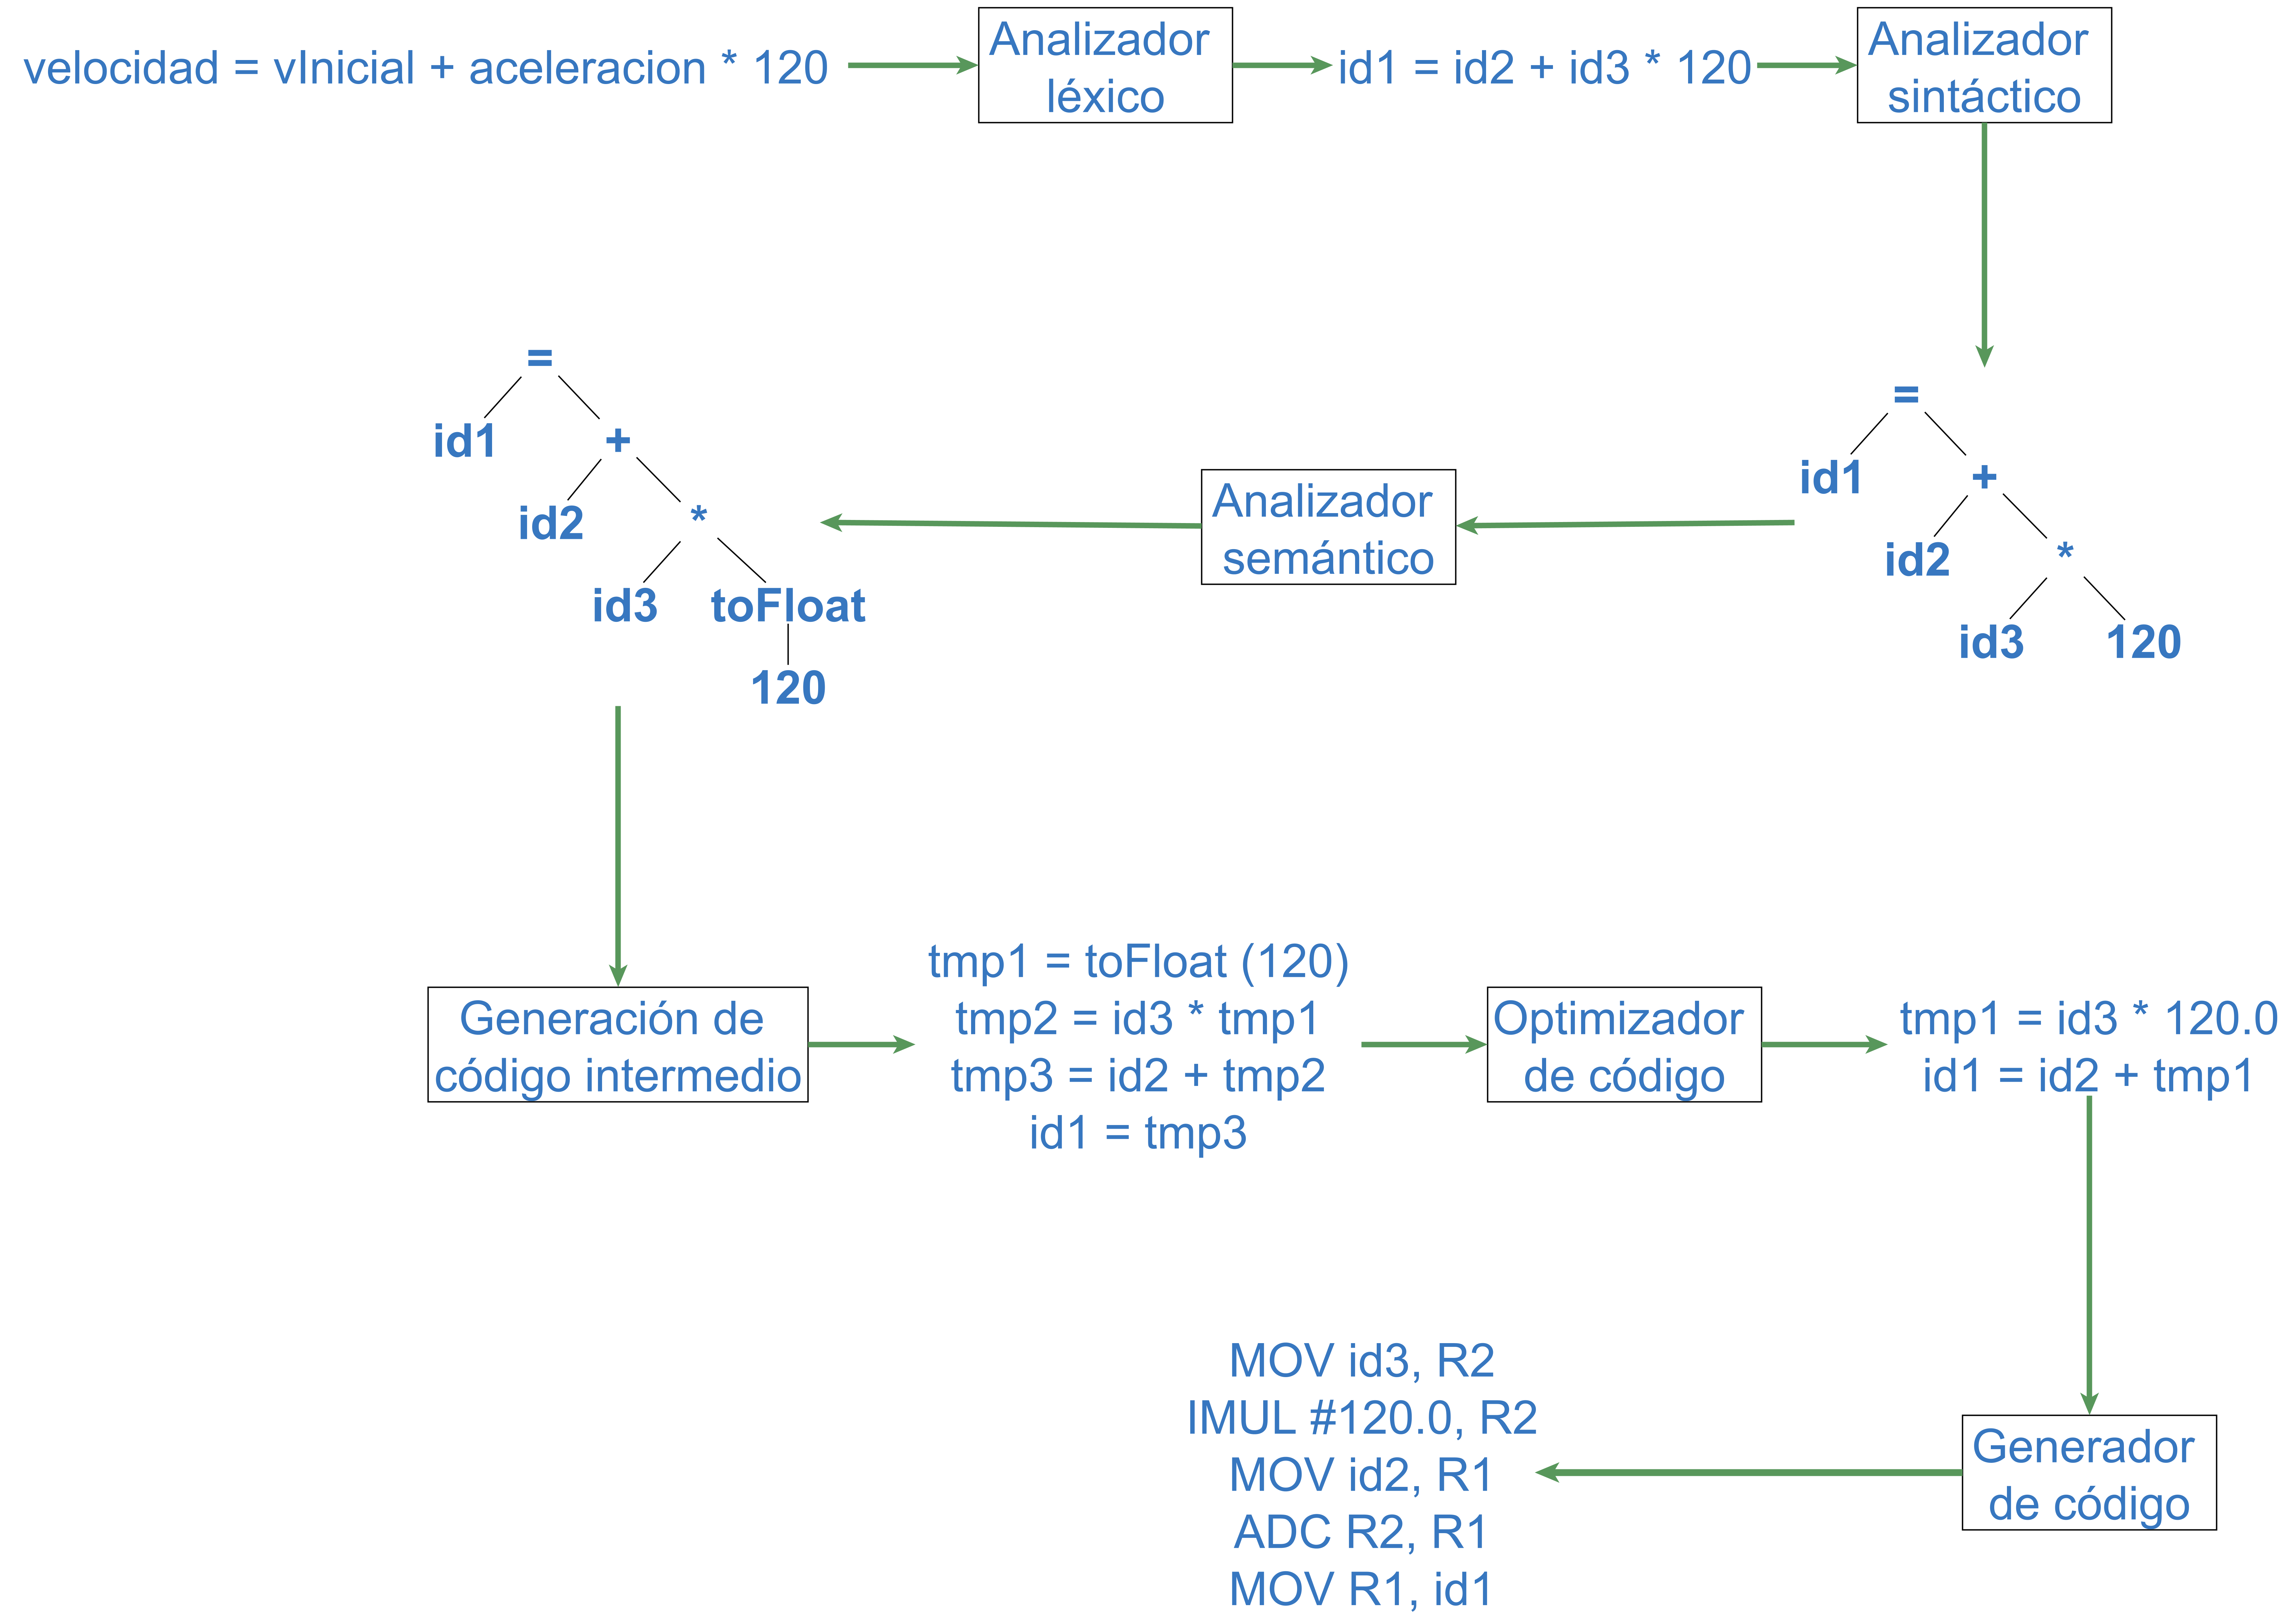
\includegraphics[width=1.0\textwidth]{imaxes/c-bases-teoricas/analisis-lexico-sintactico.png}
    \caption{Ejemplo del proceso de análisis de un compilador}
    \label{fig:analisis-lexico-sintáctico}
\end{figure}
